\documentclass[a4paper,10pt]{article}
\usepackage[utf8]{inputenc}
\usepackage[brazilian]{babel}
\usepackage{color}
\usepackage{graphicx}
\usepackage{subfig}
\usepackage[hmargin=2cm,vmargin=3.5cm,bmargin=2cm]{geometry}
\usepackage{cite}
\usepackage{float}
\usepackage{enumerate}
\usepackage{amsmath}
\usepackage{verbatim}
\usepackage{listings}
\usepackage{listingsutf8}

\definecolor{mygreen}{rgb}{0,0.6,0}
\definecolor{mygray}{rgb}{0.5,0.5,0.5}
\definecolor{mymauve}{rgb}{0.58,0,0.82}

\lstset{ %
  backgroundcolor=\color{white},   % choose the background color; you must add \usepackage{color} or \usepackage{xcolor}
  basicstyle=\footnotesize,        % the size of the fonts that are used for the code
  breakatwhitespace=false,         % sets if automatic breaks should only happen at whitespace
  breaklines=true,                 % sets automatic line breaking
  captionpos=b,                    % sets the caption-position to bottom
  commentstyle=\color{mygreen},    % comment style
  deletekeywords={...},            % if you want to delete keywords from the given language
  escapeinside={\%*}{*)},          % if you want to add LaTeX within your code
  extendedchars=true,              % lets you use non-ASCII characters; for 8-bits encodings only, does not work with UTF-8
  frame=single,	                   % adds a frame around the code
  keepspaces=true,                 % keeps spaces in text, useful for keeping indentation of code (possibly needs columns=flexible)
  keywordstyle=\color{blue},       % keyword style
  language=Octave,                 % the language of the code
  otherkeywords={*,...},            % if you want to add more keywords to the set
  numbers=left,                    % where to put the line-numbers; possible values are (none, left, right)
  numbersep=5pt,                   % how far the line-numbers are from the code
  numberstyle=\tiny\color{mygray}, % the style that is used for the line-numbers
  rulecolor=\color{black},         % if not set, the frame-color may be changed on line-breaks within not-black text (e.g. comments (green here))
  showspaces=false,                % show spaces everywhere adding particular underscores; it overrides 'showstringspaces'
  showstringspaces=false,          % underline spaces within strings only
  showtabs=false,                  % show tabs within strings adding particular underscores
  stepnumber=2,                    % the step between two line-numbers. If it's 1, each line will be numbered
  stringstyle=\color{mymauve},     % string literal style
  tabsize=2,	                   % sets default tabsize to 2 spaces
  title=\lstname                   % show the filename of files included with \lstinputlisting; also try caption instead of title
}

\begin{document}

\title{PGF 5005 - Mecânica Clássica \\ Prof. Iberê L. Caldas \\ Primeiro Estudo Dirigido \\ 2º Semestre de 2015}

\author{Aluno: Rafael M. Miller \\ NUSP.: 7581818}

\maketitle

\section*{Introdução}

\section*{Exercício 2.1.1}

  A expressão para $q^{(n+1)}$ de acordo com a equação do método de Euler (equação (2) encontrada em \cite{estudodirigido1}) é:

  \begin{equation}
    q^{(n+1)} = q^n + \Delta t \frac{\partial H}{\partial p}\Big|_{(q^{(n)},p^{(n)})} = q^n + \Delta t \; p
  \end{equation}

  Para $p^{(n+1)}$ temos:

  \begin{equation}
    p^{(n+1)} = p^n - \Delta t \frac{\partial H}{\partial q}\Big|_{(q^{(n)},p^{(n)})} = p^n + \Delta t \; sen(q)
  \end{equation}

\section*{Exercício 2.1.2}
  O programa solicitado está disposto em Anexos: Programa 1 - Equações de Euler para o pêndulo simples.

\section*{Exercício 2.1.3}
  Segue abaixo a Figura 1 solicitada no exercício.
  \begin{figure}[H]
    \centering
    \includegraphics[scale=0.6]{../Programa1/Figura1.png}
    \caption{Libração de um pêndulo simples}
  \end{figure}

  Podemos observar uma grande diferença entre os valores de $\Delta t$. Ao utilizar um valor ``alto" \; de $\Delta t$ os valores
de $q(t)$ e $p(t)$ diminuem com o passar do tempo, o que não é esperado. Ao observarmos o gráfico da Figura 5, veremos que para $\Delta t = 0.1$
o movimento se transforma para um movimento de rotação! Escolhi manter esse gráfico pois demonstra não somente uma espiral crescente, mas uma
mudança no próprio sistema físico que estamos estudando. Isso ocorre devido ao erro intrínseco do método de Euler feito dessa forma e que pode
ser contornado ao diminuirmos $\Delta t$. Veremos que o método de Euler feito no Programa 1 não é simplético, conforme discutido no Exercício
2.2.1 e que ao alterar o método para o que é descrito na equação (3) de \cite{estudodirigido1} esse erro deixará de ocorrer. Os gráficos das
Figuras 1 a 6 terão esse problema pois todos foram feitos a partir dos dados gerados pelo Programa 1.

  \begin{figure}[H]
    \centering
    \includegraphics[scale=0.6]{../Programa1/Figura2.png}
    \caption{Rotação de um pêndulo simples}
  \end{figure}

\section*{Exercício 2.1.4}

Assim como no gráfico de p(t) x t do exercício anterior, não é esperado que a energia do sistema aumente com o passar do tempo.
Isso também ocorre pelo método de Euler do Programa 1 não ser simplético.

  \begin{figure}[H]
    \centering
    \includegraphics[scale=0.6]{../Programa1/Figura3.png}
    \caption{Energia de libração do pêndulo simples}
  \end{figure}

  \begin{figure}[H]
    \centering
    \includegraphics[scale=0.6]{../Programa1/Figura4.png}
    \caption{Energia de rotação do pêndulo simples}
  \end{figure}

\section*{Exercício 2.1.5}

 Observamos das figuras de trajetórias (p(t) x q(t)) que este método só é capaz de reproduzir as órbitas esperadas
no movimento de libração para $\Delta t = 0.01$ e $\Delta t = 0.001$. Para o caso de $\Delta t = 0.1$ as linhas se abrem e
o movimento de libração (com órbita fechada) se torna um movimento de rotação devido ao aumento de energia pelo fato do método
não ser simplético. Na Figura 11 temos os gráficos de libração como o esperado, pois o método sofreu a modificação necessária.

\begin{figure}[H]
  \centering
  \includegraphics[scale=0.6]{../Programa1/Figura5.png}
  \caption{Trajetória de libração do pêndulo simples}
\end{figure}

\begin{figure}[H]
  \centering
  \includegraphics[scale=0.6]{../Programa1/Figura6.png}
  \caption{Trajetória de rotação do pêndulo simples}
\end{figure}

\section*{Exercício 2.1.6}
  O programa solicitado está disposto em Anexos: Programa 2 - Equações modificadas de Euler para o pêndulo simples.

\section*{Exercício 2.1.7}
  Seguem abaixo as Figura 7 e 8 solicitadas no exercício. Desta vez observamos o comportamento esperado para ambos
  os gráficos graças as modificações realizadas do Programa 1 para o Programa 2. Particularmente nessas duas Figuras
  solicitadas, não é possível notar uma distinção entre as curvas para os diferentes $\Delta t$. Ou seja, a diminuição
  no $\Delta t$ que servia para ``contornar" o problema do método não ser simplético não se vê mais necessária.


  \begin{figure}[H]
    \centering
    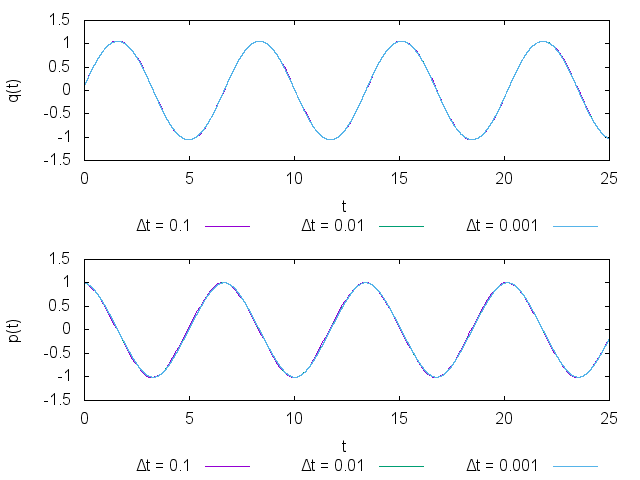
\includegraphics[scale=0.6]{../Programa2/Figura7.png}
    \caption{Libração de um pêndulo simples (versão modificada)}
  \end{figure}

  \begin{figure}[H]
    \centering
    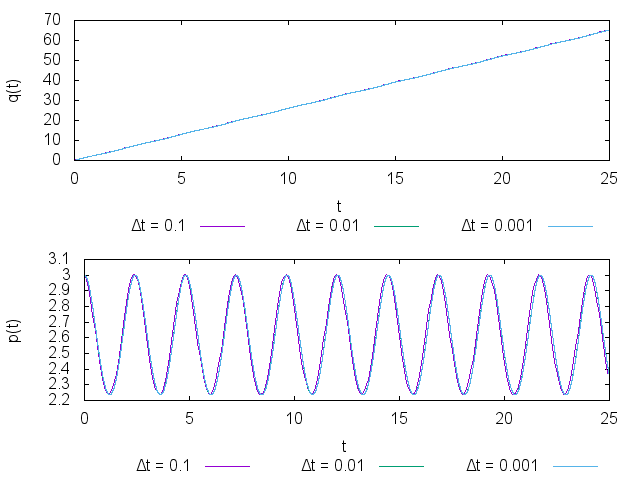
\includegraphics[scale=0.6]{../Programa2/Figura8.png}
    \caption{Rotação de um pêndulo simples (versão modificada)}
  \end{figure}

\section*{Exercício 2.1.8}

  Nos gráficos de energia para os dois movimentos do pêndulo, se percebe uma variação para cada $\Delta t$. Ao diminuir esse
  intervalo, observamos que a energia (E) se torna ``mais constante". Como a energia é uma constante desse movimento, a diminuição de sua
  variação no tempo implica na melhor representação do sistema. Apesar de não observarmos mudanças entre $\Delta t$ nos gráficos das Figuras
  7 e 8, nos gáficos das Figuras 9 e 10 essa mudança fica nítida e a importância na diminuição de $\Delta t$ para melhor representar o movimento
  se torna mais clara.

  \begin{figure}[H]
    \centering
    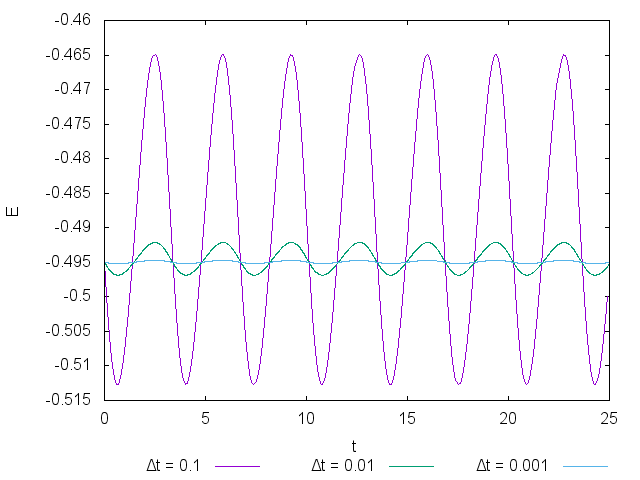
\includegraphics[scale=0.6]{../Programa2/Figura9.png}
    \caption{Energia de libração do pêndulo simples (versão modificada)}
  \end{figure}

  \begin{figure}[H]
    \centering
    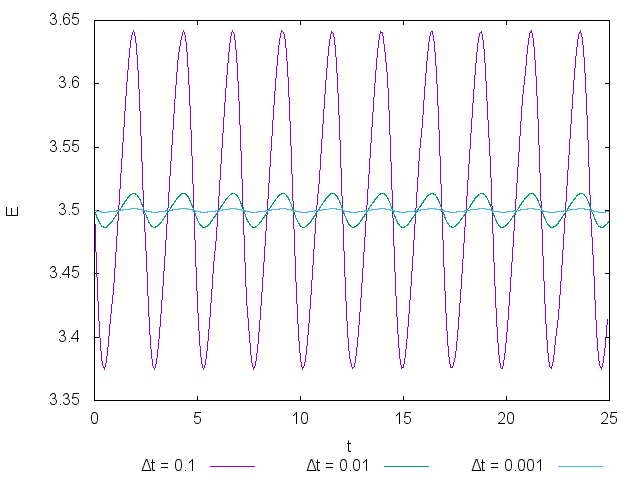
\includegraphics[scale=0.6]{../Programa2/Figura10.png}
    \caption{Energia de rotação do pêndulo simples (versão modificada)}
  \end{figure}

\section*{Exercício 2.1.9}
  Seguem abaixo as Figura 11 e 12 solicitadas no exercício. Nestes gráficos observamos o comportamento do pêndulo para os dois tipos
  de movimento. Como era esperado, a libração possui uma órbita fechada nesse gráfico de trajetória, assim como as trajetórias abertas no
  caso do movimento de rotação.

    \begin{figure}[H]
      \centering
      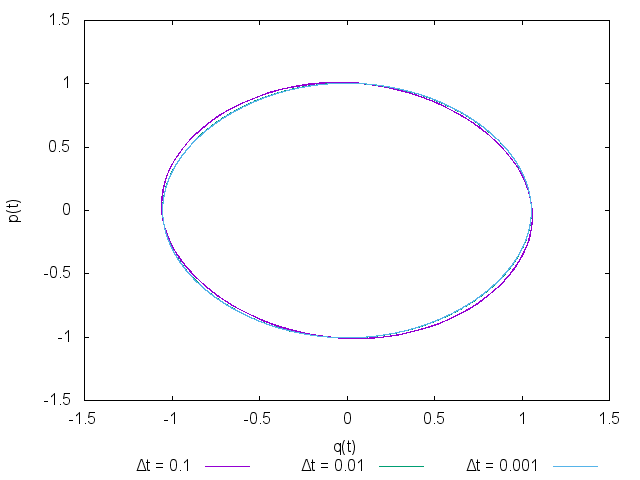
\includegraphics[scale=0.6]{../Programa2/Figura11.png}
      \caption{Trajetória de libração do simples (versão modificada)}
    \end{figure}

    \begin{figure}[H]
      \centering
      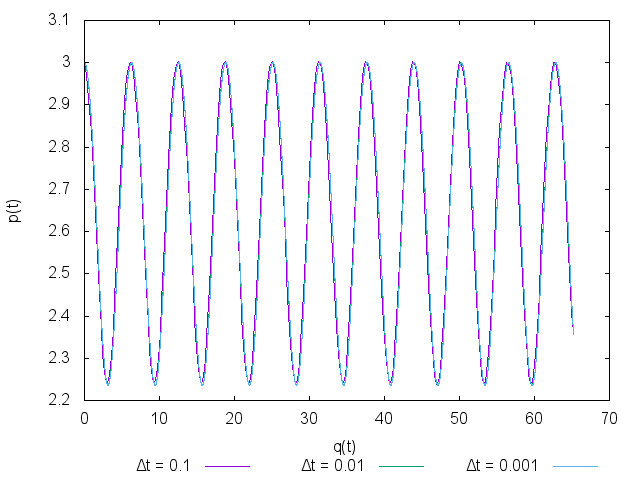
\includegraphics[scale=0.6]{../Programa2/Figura12.png}
      \caption{Trajetória de rotação do pêndulo simples (versão modificada)}
    \end{figure}

\section*{Exercício 2.2.1}

 Para verificar que um método é simplético, precisamos calcular o Jacobiano:

 \begin{equation}
   |J| = \begin{vmatrix}
            \frac{\partial p^{(n+1)}}{\partial p^{(n)}} & \frac{\partial q^{(n+1)}}{\partial p^{(n)}} \\
            \frac{\partial p^{(n+1)}}{\partial q^{(n)}} & \frac{\partial q^{(n+1)}}{\partial q^{(n)}}
         \end{vmatrix}
 \end{equation}

 Para o método de Euler, utilizando as equações (1) e (2), obtemos o seguinte Jacobiano:

 \begin{equation}
   |J| = \begin{vmatrix}
          1 & \Delta t \\
          \Delta t \; cos(q^{(n)}) & 1
         \end{vmatrix}
         = 1 - (\Delta t)^2 cos(q^{(n)})
 \end{equation}

 Observamos que esse Jacobiano é diferente de 1, o que mostra que esse método não é simplético e, por isso, carrega o erro que
 vemos nos gráficos das Figuras 1 a 6.

 Utilizando as equações para o método de Euler modificado, temos o seguinte Jacobiano:

 \begin{equation}
   |J| = \begin{vmatrix}
          1 & \Delta t \\
          0 & 1
         \end{vmatrix}
         = 1
 \end{equation}
 
 Isso implica que o método de integração modificado é simplético. Por isso temos uma melhor coerência nos gráficos das Figuras 7 a 12.

\section*{Exercício 2.3.1}

A expressão para $q^{(n+1)}$ de acordo com a equação do método de Euler (equação (2) encontrada em \cite{estudodirigido1}) é:

\begin{equation}
  q_1^{(n+1)} = q_1^n + \Delta t \frac{\partial H}{\partial p_1}\Big|_{(q_1^{(n)},p_1^{(n)},q_2^{(n)},p_2^{(n)})} = q^n + \Delta t \; p_1^n
\end{equation}

\begin{equation}
  q_2^{(n+1)} = q_2^n + \Delta t \frac{\partial H}{\partial p_2}\Big|_{(q_1^{(n)},p_1^{(n)},q_2^{(n)},p_2^{(n)})} = q^n + \Delta t \; p_2^n
\end{equation}

Para $p^{(n+1)}$ temos:

\begin{equation}
  p_1^{(n+1)} = p_1^n - \Delta t \frac{\partial H}{\partial q_1}\Big|_{(q_1^{(n+1)},p_1^{(n)},q_2^{(n+1)},p_2^{(n)})} = p_1^n + \Delta t \; (q_1^{(n+1)} + 2 q_1^{(n+1)} q_2^{(n+1)})
\end{equation}

\begin{equation}
  p_2^{(n+1)} = p_2^n - \Delta t \frac{\partial H}{\partial q_2}\Big|_{(q_1^{(n+1)},p_1^{(n)},q_2^{(n+1)},p_2^{(n)})} = p_2^n + \Delta t \; (q_2^{(n+1)} + (q_1^{(n+1)})^2 - (q_2^{(n+1)})^2)
\end{equation}

\section*{Exercício 2.3.2}
  O programa solicitado está disposto em Anexos: Programa 3 - Método de Euler simplético para a hamiltoniana de Hénon-Heiles.

\section*{Exercício 2.3.3}

  Segue abaixo o mapa de Poincaré para a Hamiltoniana de Hénon-Helies com $E = 0.08333$. Nessa figura podemos observar quatro regiões distintas
  que possuem órbitas fechadas, a separatriz dessas regiões (representada em azul claro) e em roxo a ``curva limite" para o movimento desse sistema.
  Na legenda do gráfico estão dispostas as condições iniciais de $q_2(t)$ e $p_2(t)$ utilizadas para obter as respectivas curvas.

\begin{figure}[H]
  \centering
  \includegraphics[scale=0.5]{../Programa3/Figura13.png}
  \caption{Seção de Poincaré para a Hamiltoniana de Hénon-Helies (E = 0.08333)}
\end{figure}

\section*{Exercício 2.3.4}

  Segue abaixo o mapa de Poincaré para a Hamiltoniana de Hénon-Helies com $E = 0.125$. Diferentemente da Figura 13, agora podemos observar
  o comportamento caótico desse sistema (ateriormente a energia utilizada não apresentava esse tipo de comportamento). Nas mesmas regiões em
  que observamos as órbitas para $E = 0.08333$ ocorrem as órbitas para a Figura 14, porém, temos uma região com cinco ``ilhas" que pertencem
  a uma unica órbita periódica. Também observamos um movimento quasi-periódico nos pontos em verde, que surgem muito próximos a uma separatriz
  desse sistema.

\begin{figure}[H]
  \centering
  \includegraphics[scale=0.5]{../Programa3/Figura14.png}
  \caption{Seção de Poincaré para a Hamiltoniana de Hénon-Helies (E = 0.125)}
\end{figure}

\section*{Exercício 2.3.5}

  Está disposta abaixo a Figura com os gráficos solicitados neste exercício.

\begin{figure}[H]
  \centering
  \includegraphics[scale=0.4]{../Programa3/Figura15.png}
  \caption{Trajetória regular para a Hamiltoniana de Hénon-Helies}
\end{figure}

\section*{Exercício 2.3.6}

  Está disposta abaixo a Figura com os gráficos solicitados neste exercício.

\begin{figure}[H]
  \centering
  \includegraphics[scale=0.4]{../Programa3/Figura16.png}
  \caption{Trajetória caótica para a Hamiltoniana de Hénon-Helies}
\end{figure}


\section*{Exercício 2.3.7}

  Segue abaixo o mapa de Poincaré para a Hamiltoniana de Hénon-Helies para o caso em que $E = 0.16667$. Nessa figura podemos observar um comportamento
  predominantemente caótico. Um movimento periódico ocorre em para os pontos em azul, onde surgem duas ``ilhas". Também podemos notar que ocorre um
  movimento periódico para os pontos em verde. Pontos de um movimento quasi-periódico estão em amarelo que, pela aproximação com as ``ilhas", podemos
  afirmar que estão próximos a uma separatriz do sistema.

\begin{figure}[H]
  \centering
  \includegraphics[scale=0.5]{../Programa3/Figura17.png}
  \caption{Seção de Poincaré para a Hamiltoniana de Hénon-Helies (E = 0.16667)}
\end{figure}

\begin{thebibliography}{99}

\bibitem{estudodirigido1}
Prof. Iberê L. Caldas, Primeiro Estudo Dirigido (2º Semestre de 2015) \\ http://web.if.usp.br/controle/sites/web.if.usp.br.controle/files/EstudoDirigido1.pdf

\bibitem{artigo}
Henon, M., Heiles, C., \emph{The applicability of the third integral of motion: Some numerical experiments}, Astronomical Journal, Vol. 69, p. 73 (1964)

\end{thebibliography}

\section*{Anexos}

\subsection*{Programa 1 - Equações de Euler para o pêndulo simples}
\lstset{inputencoding=utf8/latin1}
\lstinputlisting{../Programa1/programa1.cpp}

\subsection*{Programa 2 - Equações modificadas de Euler para o pêndulo simples}
\lstset{inputencoding=utf8/latin1}
\lstinputlisting{../Programa2/programa2.cpp}

\subsection*{Programa 3 - Método de Euler simplético para a hamiltoniana de Hénon-Heiles}
\lstset{inputencoding=utf8/latin1}
\lstinputlisting{../Programa3/programa3.cpp}


\end{document}
